% Created by tikzDevice version 0.12 on 2019-04-03 10:52:50
% !TEX encoding = UTF-8 Unicode
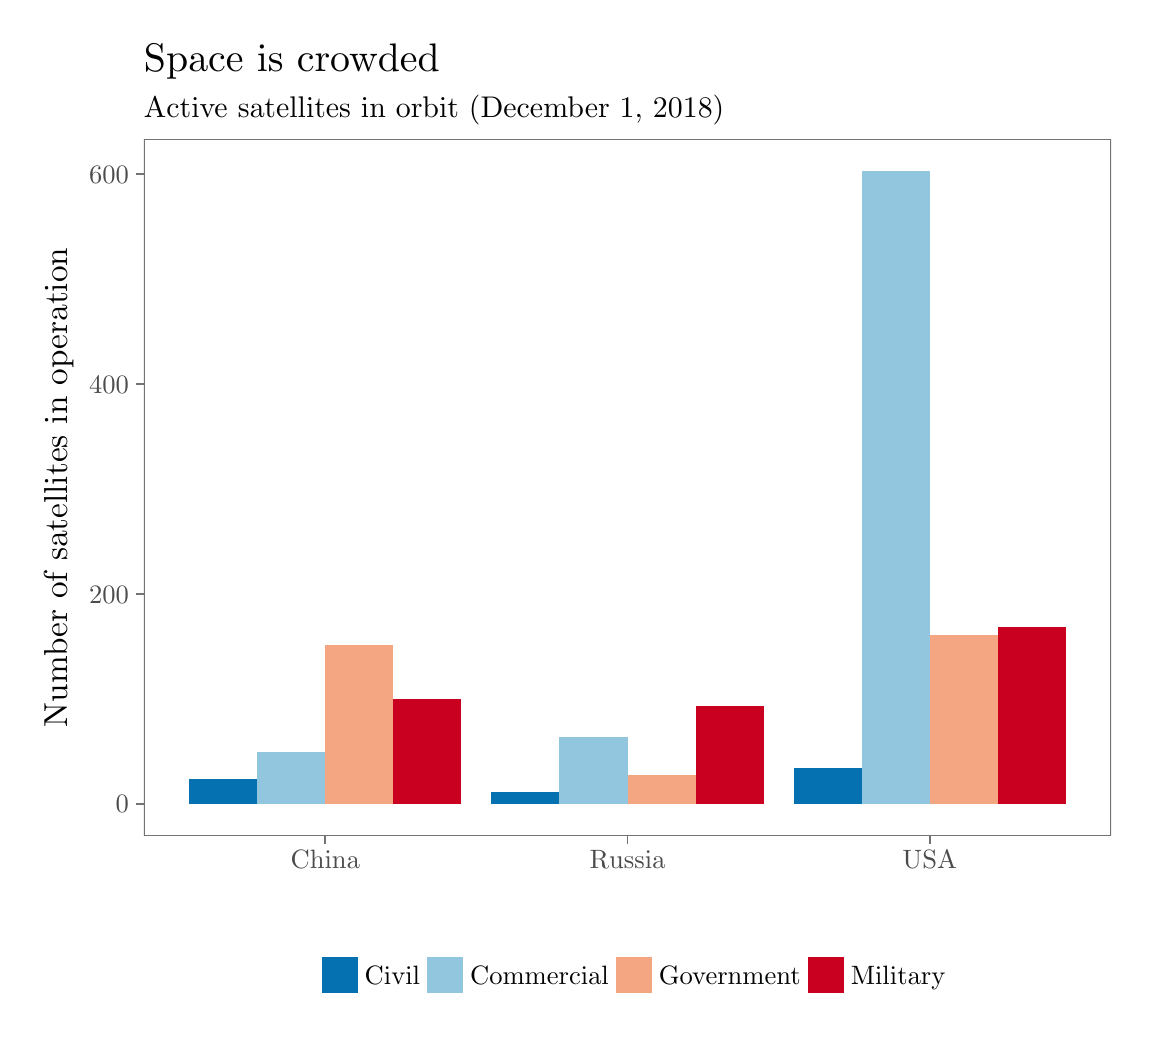
\begin{tikzpicture}[x=1pt,y=1pt]
\definecolor{fillColor}{RGB}{255,255,255}
\path[use as bounding box,fill=fillColor,fill opacity=0.00] (0,0) rectangle (397.48,361.35);
\begin{scope}
\path[clip] (  0.00,  0.00) rectangle (397.48,361.35);
\definecolor{drawColor}{RGB}{255,255,255}
\definecolor{fillColor}{RGB}{255,255,255}

\path[draw=drawColor,line width= 0.6pt,line join=round,line cap=round,fill=fillColor] (  0.00,  0.00) rectangle (397.48,361.35);
\end{scope}
\begin{scope}
\path[clip] ( 42.01, 69.49) rectangle (391.48,320.95);
\definecolor{fillColor}{RGB}{255,255,255}

\path[fill=fillColor] ( 42.01, 69.49) rectangle (391.48,320.95);
\definecolor{fillColor}{RGB}{202,0,32}

\path[fill=fillColor] (132.11, 80.92) rectangle (156.68,118.83);
\definecolor{fillColor}{RGB}{244,165,130}

\path[fill=fillColor] (107.53, 80.92) rectangle (132.11,138.17);
\definecolor{fillColor}{RGB}{146,197,222}

\path[fill=fillColor] ( 82.96, 80.92) rectangle (107.53, 99.50);
\definecolor{fillColor}{RGB}{5,113,176}

\path[fill=fillColor] ( 58.39, 80.92) rectangle ( 82.96, 90.02);
\definecolor{fillColor}{RGB}{202,0,32}

\path[fill=fillColor] (241.32, 80.92) rectangle (265.89,116.18);
\definecolor{fillColor}{RGB}{244,165,130}

\path[fill=fillColor] (216.75, 80.92) rectangle (241.32, 91.16);
\definecolor{fillColor}{RGB}{146,197,222}

\path[fill=fillColor] (192.17, 80.92) rectangle (216.75,105.19);
\definecolor{fillColor}{RGB}{5,113,176}

\path[fill=fillColor] (167.60, 80.92) rectangle (192.17, 85.09);
\definecolor{fillColor}{RGB}{202,0,32}

\path[fill=fillColor] (350.53, 80.92) rectangle (375.10,144.61);
\definecolor{fillColor}{RGB}{244,165,130}

\path[fill=fillColor] (325.96, 80.92) rectangle (350.53,141.96);
\definecolor{fillColor}{RGB}{146,197,222}

\path[fill=fillColor] (301.38, 80.92) rectangle (325.96,309.52);
\definecolor{fillColor}{RGB}{5,113,176}

\path[fill=fillColor] (276.81, 80.92) rectangle (301.38, 93.81);
\definecolor{drawColor}{gray}{0.45}

\path[draw=drawColor,line width= 0.6pt,line join=round,line cap=round] ( 42.01, 69.49) rectangle (391.48,320.95);
\end{scope}
\begin{scope}
\path[clip] (  0.00,  0.00) rectangle (397.48,361.35);
\definecolor{drawColor}{gray}{0.30}

\node[text=drawColor,anchor=base east,inner sep=0pt, outer sep=0pt, scale=  0.96] at ( 36.61, 77.62) {0};

\node[text=drawColor,anchor=base east,inner sep=0pt, outer sep=0pt, scale=  0.96] at ( 36.61,153.44) {200};

\node[text=drawColor,anchor=base east,inner sep=0pt, outer sep=0pt, scale=  0.96] at ( 36.61,229.26) {400};

\node[text=drawColor,anchor=base east,inner sep=0pt, outer sep=0pt, scale=  0.96] at ( 36.61,305.08) {600};
\end{scope}
\begin{scope}
\path[clip] (  0.00,  0.00) rectangle (397.48,361.35);
\definecolor{drawColor}{gray}{0.45}

\path[draw=drawColor,line width= 0.6pt,line join=round] ( 39.01, 80.92) --
	( 42.01, 80.92);

\path[draw=drawColor,line width= 0.6pt,line join=round] ( 39.01,156.74) --
	( 42.01,156.74);

\path[draw=drawColor,line width= 0.6pt,line join=round] ( 39.01,232.56) --
	( 42.01,232.56);

\path[draw=drawColor,line width= 0.6pt,line join=round] ( 39.01,308.38) --
	( 42.01,308.38);
\end{scope}
\begin{scope}
\path[clip] (  0.00,  0.00) rectangle (397.48,361.35);
\definecolor{drawColor}{gray}{0.45}

\path[draw=drawColor,line width= 0.6pt,line join=round] (107.53, 66.49) --
	(107.53, 69.49);

\path[draw=drawColor,line width= 0.6pt,line join=round] (216.75, 66.49) --
	(216.75, 69.49);

\path[draw=drawColor,line width= 0.6pt,line join=round] (325.96, 66.49) --
	(325.96, 69.49);
\end{scope}
\begin{scope}
\path[clip] (  0.00,  0.00) rectangle (397.48,361.35);
\definecolor{drawColor}{gray}{0.30}

\node[text=drawColor,anchor=base,inner sep=0pt, outer sep=0pt, scale=  0.96] at (107.53, 57.48) {China};

\node[text=drawColor,anchor=base,inner sep=0pt, outer sep=0pt, scale=  0.96] at (216.75, 57.48) {Russia};

\node[text=drawColor,anchor=base,inner sep=0pt, outer sep=0pt, scale=  0.96] at (325.96, 57.48) {USA};
\end{scope}
\begin{scope}
\path[clip] (  0.00,  0.00) rectangle (397.48,361.35);
\definecolor{drawColor}{RGB}{1,2,2}

\node[text=drawColor,rotate= 90.00,anchor=base,inner sep=0pt, outer sep=0pt, scale=  1.20] at ( 14.26,195.22) {Number of satellites in operation};
\end{scope}
\begin{scope}
\path[clip] (  0.00,  0.00) rectangle (397.48,361.35);
\definecolor{fillColor}{RGB}{255,255,255}

\path[fill=fillColor] ( 96.23,  6.00) rectangle (337.26, 31.84);
\end{scope}
\begin{scope}
\path[clip] (  0.00,  0.00) rectangle (397.48,361.35);
\definecolor{fillColor}{RGB}{255,255,255}

\path[fill=fillColor] (105.53, 11.69) rectangle (119.99, 26.14);
\end{scope}
\begin{scope}
\path[clip] (  0.00,  0.00) rectangle (397.48,361.35);
\definecolor{fillColor}{RGB}{5,113,176}

\path[fill=fillColor] (106.24, 12.40) rectangle (119.27, 25.43);
\end{scope}
\begin{scope}
\path[clip] (  0.00,  0.00) rectangle (397.48,361.35);
\definecolor{fillColor}{RGB}{255,255,255}

\path[fill=fillColor] (143.59, 11.69) rectangle (158.05, 26.14);
\end{scope}
\begin{scope}
\path[clip] (  0.00,  0.00) rectangle (397.48,361.35);
\definecolor{fillColor}{RGB}{146,197,222}

\path[fill=fillColor] (144.31, 12.40) rectangle (157.34, 25.43);
\end{scope}
\begin{scope}
\path[clip] (  0.00,  0.00) rectangle (397.48,361.35);
\definecolor{fillColor}{RGB}{255,255,255}

\path[fill=fillColor] (211.81, 11.69) rectangle (226.26, 26.14);
\end{scope}
\begin{scope}
\path[clip] (  0.00,  0.00) rectangle (397.48,361.35);
\definecolor{fillColor}{RGB}{244,165,130}

\path[fill=fillColor] (212.52, 12.40) rectangle (225.55, 25.43);
\end{scope}
\begin{scope}
\path[clip] (  0.00,  0.00) rectangle (397.48,361.35);
\definecolor{fillColor}{RGB}{255,255,255}

\path[fill=fillColor] (281.16, 11.69) rectangle (295.61, 26.14);
\end{scope}
\begin{scope}
\path[clip] (  0.00,  0.00) rectangle (397.48,361.35);
\definecolor{fillColor}{RGB}{202,0,32}

\path[fill=fillColor] (281.87, 12.40) rectangle (294.90, 25.43);
\end{scope}
\begin{scope}
\path[clip] (  0.00,  0.00) rectangle (397.48,361.35);
\definecolor{drawColor}{RGB}{1,2,2}

\node[text=drawColor,anchor=base west,inner sep=0pt, outer sep=0pt, scale=  0.96] at (121.79, 15.61) {Civil};
\end{scope}
\begin{scope}
\path[clip] (  0.00,  0.00) rectangle (397.48,361.35);
\definecolor{drawColor}{RGB}{1,2,2}

\node[text=drawColor,anchor=base west,inner sep=0pt, outer sep=0pt, scale=  0.96] at (159.86, 15.61) {Commercial};
\end{scope}
\begin{scope}
\path[clip] (  0.00,  0.00) rectangle (397.48,361.35);
\definecolor{drawColor}{RGB}{1,2,2}

\node[text=drawColor,anchor=base west,inner sep=0pt, outer sep=0pt, scale=  0.96] at (228.07, 15.61) {Government};
\end{scope}
\begin{scope}
\path[clip] (  0.00,  0.00) rectangle (397.48,361.35);
\definecolor{drawColor}{RGB}{1,2,2}

\node[text=drawColor,anchor=base west,inner sep=0pt, outer sep=0pt, scale=  0.96] at (297.42, 15.61) {Military};
\end{scope}
\begin{scope}
\path[clip] (  0.00,  0.00) rectangle (397.48,361.35);
\definecolor{drawColor}{RGB}{1,2,2}

\node[text=drawColor,anchor=base west,inner sep=0pt, outer sep=0pt, scale=  1.08] at ( 42.01,328.85) {Active satellites in orbit (December 1, 2018)};
\end{scope}
\begin{scope}
\path[clip] (  0.00,  0.00) rectangle (397.48,361.35);
\definecolor{drawColor}{RGB}{1,2,2}

\node[text=drawColor,anchor=base west,inner sep=0pt, outer sep=0pt, scale=  1.44] at ( 42.01,345.43) {Space is crowded};
\end{scope}
\end{tikzpicture}
